\section*{Results}

\subsection*{Data Exploration}

\subsubsection*{Data Reduction}

The data taken from the Census Bureau has one row per person, containing approximately 3.2 million observations. This was obviously far too large for a bayesian analysis so a lot of data reduction was done. For starters, 800k rows were removed that had the educational category "NIU" or "Not In Universe". This was the only column that had any "missing" data and I felt it best to narrow down to the subset of the data that fell into the remaining educational categories. 

After this, I performed stratified sampling on the categorical covariates. This was done to ensure that the same ratios for all of the categories are maintained while reducing the row count. This process is extremely important when working with many unbalanaced categories, especially when doing a row reduction as extreme as what I am doing. I used a proportion of $0.005$ to bring the sample size down to around 11000 rows. Without stratified sampling I likely would have lost many of the entire categories I need to keep for my analysis. So with this I have a far more manageable dataset that at least maintains the information in the categorical covariates.

\begin{table}[ht]
\centering
\begin{tabular}{|l|p{7cm}|l|}
\hline
\textbf{Variable} & \textbf{Description} & \textbf{Variable Type} \\
\hline
\texttt{spm\_poor} & Poverty status under SPM & Binary \\
\texttt{spm\_povthreshold} & SPM poverty threshold for the unit & Continuous \\
\texttt{region} & Region of residence & Categorical \\
\texttt{age} & Age of individual & Continuous \\
\texttt{mar} & Married & boolean \\
\texttt{sex\_female} & Is individual female & binary \\
\texttt{education} & Educational attainment & Categorical \\
\texttt{race} & Race & Categorical \\
\texttt{hispanic} & Hispanic ethnicity & Binary \\
\texttt{agi} & Adjusted gross income & Continuous \\
\texttt{hi\_premium} & Health insurance premium & Continuous\\
\texttt{moop\_other} & Medical out-of-pocket expenses & Continuous \\
\hline
\end{tabular}
\caption{Variable Descriptions and Types}
\label{tab:variables}
\end{table}


\subsubsection*{Response Variable: spm\_poor}

To start we will look at our response variable which represents a simple yes or no indicator on whether an individual is classified as poor by the SPM. All there really is to see here is a poverty rate of around 13\%, roughly matching the Bureau's own reported numbers for the SPM. With boolean variables such as this there isn't a ton to say so that just about covers it. What'll be more interesting is seeing how it relates to other variables.

\subsubsection*{Covariate Candidates}

Note that the below tables are created using only values from the stratified dataframe.

\begin{table}[h!]
\centering
\begin{tabular}{|l|c|c|c|c|c|c|}
\hline
\rowcolor[HTML]{E7EAF6} 
\multicolumn{1}{|c|}{\textbf{Covariate}} & \multicolumn{1}{c|}{Min} & \multicolumn{1}{c|}{1st Quartile} & \multicolumn{1}{c|}{Mean} & \multicolumn{1}{c|}{Median} & \multicolumn{1}{c|}{3rd Quartile} & \multicolumn{1}{c|}{Max} \\ \hline
Pov Threshold & 11420 & 18236 & 26805 & 23626 & 33282 & 113199 \\ \hline
Age & 25 & 40 & 54.2 & 55 & 67 & 96 \\ \hline
AGI & -5000 & 19966 & 89629 & 60000 & 118000 & 1520000 \\ \hline
HI Premium & 0 & 0 & 1782 & 540 & 2400 & 70259 \\ \hline
MOOP & 0 & 151 & 1302 & 500 & 1375 & 54586 \\ \hline
\end{tabular}
\caption{Summary of numeric candidates.}
\end{table}


\begin{table}[h!]
\centering
\begin{tabular}{|l|c|p{8cm}|}
\hline
\rowcolor[HTML]{E7EAF6} 
\textbf{Covariate} & \textbf{\# Levels} & \textbf{Most Common Levels (Count)} \\ \hline
Education & 4 & \textbf{C}: 4246, \textbf{SC}: 3155, \textbf{HS}: 2887, \textbf{$<$HS}: 966 \\ \hline
Race & 4 & \textbf{Wh}: 8058, \textbf{Oth}: 1685, \textbf{Bl}: 852, \textbf{Asi}: 659 \\ \hline
Region & 4 & \textbf{S}: 4335, \textbf{W}: 2623, \textbf{MidW}: 2346, \textbf{NE}: 1950 \\ \hline
\end{tabular}
\caption{Summary of categorical candidates.}
\end{table}


\begin{table}[h!]
\centering
\begin{tabular}{|l|c|c|}
\hline
\rowcolor[HTML]{E7EAF6} 
\multicolumn{1}{|c|}{\textbf{Covariate}} & \multicolumn{1}{c|}{TRUE} & \multicolumn{1}{c|}{FALSE}\\ \hline
Hispanic & 1379 & 9875 \\ \hline
Married & 6864 & 4390 \\ \hline
Female & 5914 & 5340 \\ \hline
\end{tabular}
\caption{Summary of boolean candidates.}
\end{table}


For this project I have quite a number of possible covariates to include and a lot of variation in data types as well. 

Looking at our numeric candidates first, all of them have radically different scales and distributions. None of them are normal, not even close. Health insurance premium and medical out of pocket expenses both have nearly all of their density at 0 and then comically long tails. I think it would be extremely generous to even think of these as log-normal. I was immediately concerned about my ability to make these two candidates work. Adjusted gross income and the spm poverty threshold have a lot more variety going on in their distributions at least; they're both either bi-modal or multi-modal with a far right tail with AGI having a far more extreme maximum. Lastly, age is a lot more calm. It's more of a demographic variable so it's fairly even in density across the board with a steep dropoff after 75. To account for all of this variety I considered scaling all of these variables but I didn't want to deal with the additional issues with interpretation problems so I kept them as is. We will discuss this decision more later.

As for our categorical and boolean candidates, those are a lot easier to write about. Starting with married, it used to be marital status. However, it was extremely unbalanced and I wanted to keep the information from those smaller categories like divorced, widowed and separated. Similarly, region used to be state. Bringing that from 50 down to 4 categories is far more manageable, especially for stratified sampling. As for relationships to the response variable, the big one that jumps out to me is education. Less than a high school degree has a far larger proportion of those in poverty than the other options. So at first glance I would assume that candidate would end up mattering a lot. 

\subsection*{Variable and Model Selection}

For variable selection I initially tried a LASSO method. The goal here was to start with the full model and let the lasso penalty drag unnecessary covariates to zero. This method allowed me to greatly reduce the complexity of the model without hindering performance. However, two things got in the way of that at the last minute. The most important thing is that I made an enormous mistake. As of writing this report, I noticed that I had somehow forgot to include the binomial family in my rstanarm code. Rstanarm had been treating what I thought of as a logistic regression with a gaussian family. On top of that, fixing that little mixup caused the lasso regression to no longer work. It mostly just got stuck. So in my panic I have a new, sloppy, variable selection method to discuss. 

For my new and hastily thrown together method, I simply ran the model and looked for possible candidates for removal. Any of the intervals that straddled or appeared extremely close to 0 were removed. I created 3 models this way. The first model is the full one and I noticed that I could potentialy removed some of the messier numeric columns. So for the second model I got rid of health insurance premium, AGI, out of pocket medical expenses and age. From here I removed hispanic as it is highly correlated with race\_other. 

To compare the 3 models I looked at their WAIC scores and $R_b^2$ which are shown below. What shocked me was the drastic difference in model performance. Under my original and incorrect method this barely changed anything, but here we see the performance drop off of a cliff instantly. It is worth pointing out here that I did attempt running these models with the numeric variables scaled and their importance becomes far more obvious. For the sake of this project that is now falling apart at the seams I decided to keep them unscaled as it leads to some more interesting results and decisions. 

\begin{table}[h!]
\centering
\begin{tabular}{|l|c|c|}
\hline
\rowcolor[HTML]{E7EAF6} 
\textbf{Model} & \textbf{WAIC} & \textbf{Standard Error} \\ \hline
Model 1 (Full) & 4931.8 & 96.3 \\ \hline
Model 2 & 7310 & 132.1  \\ \hline
Model 3 & 7308.6 & 132.1  \\ \hline
\end{tabular}
\caption{Model Scores}
\end{table}


\begin{figure}[ht!]%
    \centering
    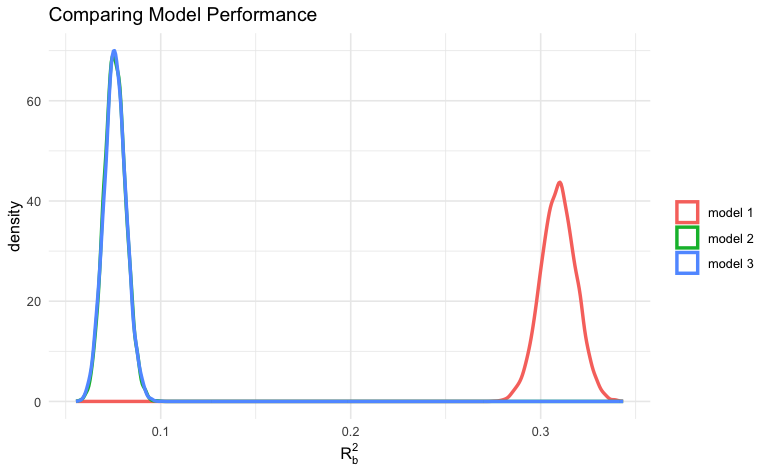
\includegraphics[width=0.8\columnwidth]{../presentation/images/rbsquared.png}
    \caption{$B_b^2$ Density Plot}%
    \label{fig:example}%
\end{figure}

So it goes without saying that I stuck with the full model here.

\subsection*{Model Assessment}

When checking the model, I was primarily interested in convergence diagnostics. I wanted to see whether any of the covariates exhibited strange behavior or failed to explore their parameter space effectively. I created several diagnostic plots, and all appeared well-behaved.

For the trace plots, the chains looked dense and well-mixed, with no obvious signs of them getting stuck or failing to explore the posterior. The posterior violin plots looked good too. For these, we expect the violins from different chains to have similar shapes and no unusual or highly skewed distributions. This is exactly what we got which is good.

I also examined the autocorrelation plots. These showed a steep drop off, suggesting low autocorrelation and good mixing across all covariates.

\begin{figure}[ht!]%
    \centering
    \subfloat[\centering Trace Plots]{{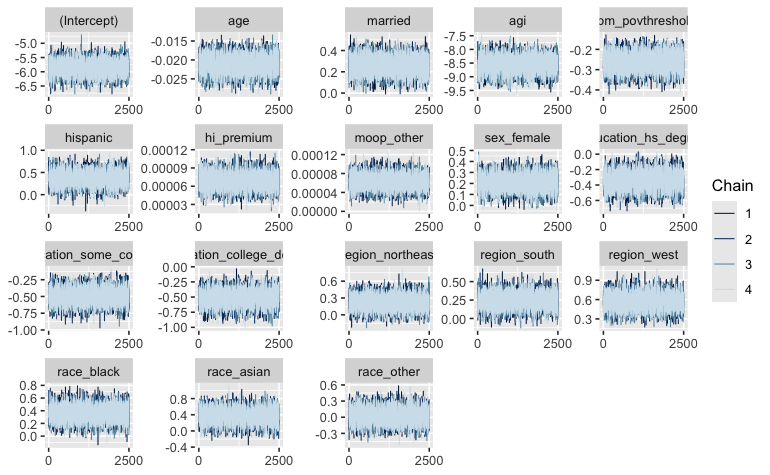
\includegraphics[width=7cm]{../presentation/images/trace-plots.png} }}%
    \qquad
    \subfloat[\centering Violin Plots]{{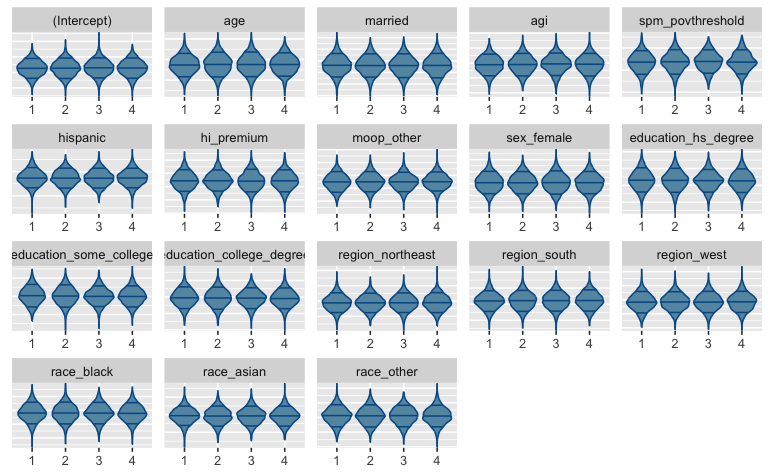
\includegraphics[width=7cm]{../presentation/images/violins_updated.png} }}%
    \caption{Model Assessment Examples}%
    \label{fig:example}%
\end{figure}

\subsection*{Final Model and Coefficient Interpretation}

\begin{table}[h!]
\centering
\begin{tabular}{|l|c|c|c|c|}
\hline
\rowcolor[HTML]{E7EAF6}
\textbf{Covariate} & \textbf{Mean} & \textbf{5\%} & \textbf{95\%} & \textbf{Relation to 1} \\ \hline
(Intercept)              & 3.77833  & 2.64188 & 5.42084 & Above \\ \hline
age                      & 0.97903  & 0.97536 & 0.98271 & Below \\ \hline
married                  & 1.29719  & 1.14371 & 1.47316 & Above \\ \hline
agi                      & 0.99992  & 0.99992 & 0.99993 & Below \\ \hline
spm\_povthreshold         & 0.99998  & 0.99997 & 0.99998 & Below \\ \hline
hispanic                 & 1.45169  & 1.12085 & 1.88613 & Above \\ \hline
hi\_premium               & 1.00007  & 1.00005 & 1.00009 & Above \\ \hline
moop\_other               & 1.00006  & 1.00004 & 1.00009 & Above \\ \hline
sex\_female               & 1.23250  & 1.09489 & 1.38985 & Above \\ \hline
education\_hs\_degree      & 0.71205  & 0.59852 & 0.84880 & Below \\ \hline
education\_some\_college   & 0.60940  & 0.50724 & 0.73408 & Below \\ \hline
education\_college\_degree & 0.59683  & 0.48618 & 0.73218 & Below \\ \hline
region\_northeast         & 1.24877  & 1.01936 & 1.53665 & Above \\ \hline
region\_south             & 1.27648  & 1.08145 & 1.51053 & Above \\ \hline
region\_west              & 1.76111  & 1.45638 & 2.13829 & Above \\ \hline
race\_black               & 1.43318  & 1.17342 & 1.74935 & Above \\ \hline
race\_asian               & 1.45619  & 1.08720 & 1.92860 & Above \\ \hline
race\_other               & 1.02326  & 0.80546 & 1.29865 & Straddles \\ \hline
\end{tabular}
\caption{95\% Credible Intervals for Model Covariate Odds Ratios: $\exp(\beta_i)$}
\end{table}


Now that we know our final model seems to be well behaved we can discuss the actual results it has provided. Let's take a look at the posterior credible intervals. The table provided shows all of the intervals taken out of the log scale. So what we're looking for is whether an interval is above or below 1 as that will indicate to us how to interpret its effect. 

Let us start with the intervals below 1. These covariates decrease the odds of being classified as in poverty by the supplemental poverty measure. The covariates here are age, adjusted gross income, spm poverty threshold, and all of the education categories with respect to the reference category. 

For age, we see a reduction of $2.1\%[1.7\%, 2.5\%]$ in the odds of being classified as in poverty per year increase. An important note here is that this type of relationship is not additive. This coefficient does not imply that someone who is 50 has 0 odds of being in poverty. This simply means that, given all other variables kept static, that someone who is older has lower odds of being classified as in poverty than someone who is younger.

AGI and poverty threshold I won't go into too much detail about. Their coefficients seem extremely non-impactful, however we need to remember their values can get very large. The general interpretation is that as someones adjusted gross income and the poverty threshold assigned to them by the spm go up dollar by dollar, that their odds of being classified as in poverty decreases. 

As for education, all of these categories reduce the odds of poverty classification quite a lot when compared to someone with less than a high school degree. For those with a high school degree, we see a reduction of $29\%[15\%, 40\%]$. Similarly, we see reductions of $39\%[27\%, 49\%]$ and $40\%[27\%, 51\%]$ for some college and college degree respectively. Interestingly, some college and a college degree overlap almost entirely under this model. In my old model college degree was quite a bit more impactful.

The ones above 1 are quite interesting. Married in particular jumps out to me. The coefficient indicates an increase of $30\%[14\%, 47\%]$ in the odds of being classified as in poverty. What's so weird about this is every other model I have fit has married comfortably below 1. For reference, model 2 (a simplified version of this model) has married showing a decrease of around $65\%$ in the odds. This final model showing an increase in the odds is very shocking to me both mathematically and practically. Even looking at a bar plot of this variable, there is a far higher proportion of those classified as in poverty in the not married category. I'm really not sure what's going on here. 

Medical out of pocket expenses and health insurance premium are similar to agi and poverty threshold yet these increase the odds of a poverty classification as they increase. Again, these coefficients seem extremely close to 1 but these variables get large enough that they still have a large impact when you start reaching realistic values. 

For our binary variables, being female shows an increase in the odds of a poverty classification by $23\%[9\%, 39\%]$. Of note that this increase is a large jump from my older non-logistic regression models. This one used to be a small enough impact that I just removed it entirely. As for hispanic, we have an extremely large interval. We see an increase in the odds of a poverty classification by $45\%[12\%, 89\%]$. It is worth noting that this large interval is likely due in part to its correlation to race\_other and them fighting over their impact. 

For region, the reference category being used is the midwest. So all of the odds ratio changes are with respect to that. We see a ranking of west, south, northeast in terms of their increases in the odds of a poverty classification with west having the highest increase of $76\%[46\%, 114\%]$ when compared to the midwest. I think many would assume that the south would have the highest increase in these odds however it is just slightly higher than the northeast showing of $28\%[8\%, 51\%]$ in the odds of a poverty classification when compared to the midwest.

Lastly we have race which has white as the reference category. All the categories excluding other show an increase in the odds of a poverty classification. Black shows an increase of $43\%[17\%, 75\%]$ and asian shows an increase of $46\%[9\%, 93\%]$. I believe it's worth pointing out that the large interval of asian. This is surprising due to it having a similar sample size in the final dataset as black with $n=659$ and $n=852$ respectively. As for the other category, this one straddles 1 but this almost certainly due to its correlation to hispanic. Models with an without hispanic shift its distribution quite a lot. 